\section{Reviewer 1}

\subsection{Question 1}
\begin{reviewcomment}
Some aspects of the architecture lack a clear justification. FluxArch uses 8 compute tiles, each containing 8 clusters with 16 cores each, but the rationale behind this organization is not explained. Was this hierarchy derived from design-space exploration or empirical evaluation? How would a different hierarchy (For example, 16 -{}> 8 -{}> 8 instead of 8 -{}> 8 -{}> 16) perform?
\end{reviewcomment}

We sincerely thank you for your helpful and constructive suggestion.

\begin{enumerate}[label=(\arabic*)]
\setlength{\emergencystretch}{1em}
\item \textbf{Hierarchy sizing.} Our hierarchy is selected bottom-up through empirical evaluation. We added hierarchy-configuration sweeps under a common requirement that every workload retain at least 80\% scaling efficiency. The results select 16 cores per cluster and eight clusters per Compute Tile as the largest sharing domains satisfying this criterion across all five workloads, yielding a 128-core tile and a 1,024-core system.

\revisionlocation{The selected hierarchy and its link to the sizing study are summarized in \textbf{Section 4.1}.}

\excerptlabel{Original (Section 4.1, page 9):}\par
\begin{manuscriptexcerpt}
\graysentence{Sixteen \name\ Cores form a \name\ Cluster, which shares a cache and TLB.} \graysentence{Eight \name\ Clusters form a \name\ Tile, which is equipped with a multi-channel memory controller optimized for bandwidth-intensive MCPT applications like XSBench.} \graysentence{At the top level, the system comprises eight Compute Tiles and a centralized Switch Tile.} \graysentence{As shown in Table~1, we carefully balanced cache capacity against the large database requirements of MCPT to optimize area.} \graysentence{A key architectural departure in \name\ is the omission of a shared L3 cache.} \graysentence{Prior analysis indicates that expanding cluster-local L2 capacity offers superior performance-per-area and reduces coherence complexity compared to a monolithic L3.} \graysentence{This design aligns with throughput-oriented architectures that prioritize L2 proximity for massive TLP, making \name\ more GPU-like while retaining independent control flows.}
\end{manuscriptexcerpt}
\excerptlabel{Revised (Section 4.1, page 8):}\par
\begin{manuscriptexcerpt}
\redsentence{We size the hierarchy bottom-up using an empirical criterion that every evaluated workload must retain at least 80\% scaling efficiency.} \redsentence{The sweeps in Section~6.6 select 16 cores per cluster and 8 clusters per Compute Tile, yielding a 128-core tile.} \redsentence{Eight such tiles are interconnected through a centralized Switch Tile to form a 1,024-core system.}
\end{manuscriptexcerpt}
\item \textbf{Alternative hierarchy configurations.} We also added direct evaluations of the $16\times8\times8$ organization, together with $32\times4\times8$ and $32\times8\times4$, while holding the total core count at 1,024, the memory system at 32 channels, and every crossbar (XBar) at no more than 64 endpoints. The revised evaluation shows geometric-mean performance of 1.00, 0.96, 0.93, and 0.89 for these four organizations, respectively. The selected $8\times8\times16$ organization performs best overall because fewer cluster-bound MPI processes preserve communication locality for CORAL2-P1, CORAL2-P2, CTS2 and Homogeneous, while the alternatives benefit XSBench through greater aggregate cluster-local level-2 (L2) cache capacity and bandwidth.
\revisionlocation{The design-space constraints, bottom-up sweeps, and alternative-hierarchy trade-offs are explained in \textbf{Section 6.6}.}

\excerptlabel{Added (Section 6.6, pages 19--20):}\par
\begin{manuscriptexcerpt}
\redsentence{We first constrain the design space in three ways.} \redsentence{We cap each XBar at 64 endpoints to avoid impractical arbitration, wiring, and timing complexity.} \redsentence{We fix both the system scale at 1,024 cores and the memory system at 32 channels, so alternative hierarchies have identical compute and off-chip bandwidth resources.} \redsentence{Within this space, we require every workload to retain at least 80\% scaling efficiency and size the sharing domains from the bottom up.} \redsentence{Fig.~17(a) varies the number of cores per cluster: 16 cores retain 81.46\%--97.98\% efficiency, whereas at 32 cores four workloads fall below the criterion.} \redsentence{Fig.~17(b) then fixes 16-core clusters and varies the number of clusters per tile: eight clusters retain 81.02\%--94.93\%, whereas at 16 clusters only CTS2 remains above 80\%.} \redsentence{These sweeps establish 16 cores per cluster and eight clusters per tile as the largest per-level configurations that satisfy the criterion across all workloads, while smaller configurations remain viable alternatives.}

\redsentence{We next compare $8\times8\times16$ against three representative alternatives that also satisfy these constraints: $16\times8\times8$, $32\times4\times8$, and $32\times8\times4$, which progressively distribute the same 1,024 cores across more, smaller sharing domains.} \redsentence{Fig.~17(c) reports geometric-mean normalized performance of 1.00, 0.96, 0.93, and 0.89 for these four configurations, respectively.} \redsentence{The per-workload results reveal two opposing effects.} \redsentence{For CORAL2-P1, CORAL2-P2, CTS2 and Homogeneous, performance declines as the number of cluster-bound MPI processes rises from 64 to 128, 128, and 256.} \redsentence{More process boundaries increase communication overhead, which is material because particle exchange already accounts for 16.93\%--31.80\% of cycle-tracking time in Table~6(c).} \redsentence{XSBench has no inter-process particle exchange and instead benefits from the higher aggregate capacity and bandwidth of 128, 128, and 256 cluster-local L2s.} \redsentence{This sensitivity agrees with Table~6(a), where XSBench has the largest database, lowest L2 read hit rate, and highest normalized DRAM read traffic.} \redsentence{Thus, $8\times8\times16$ best balances communication locality and aggregate L2 resources across the workload suite.}
\end{manuscriptexcerpt}
\par\noindent\begin{minipage}{\linewidth}
\revisionlocation{The per-level scaling sweeps and normalized alternative-hierarchy results are added in \textbf{Figure~17(a--c)}.}

\excerptlabel{Added (Figure~17, page 19):}\par
% Revised manuscript: Figure 17
\begin{figure}[H]
  \centering
  \fbox{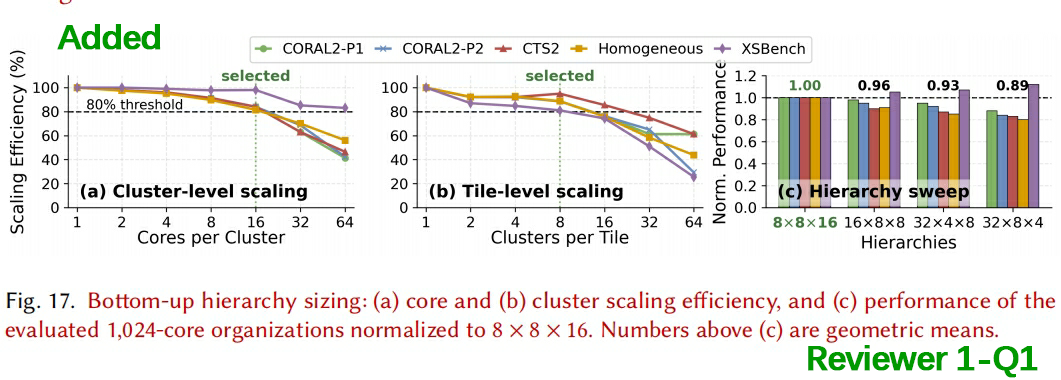
\includegraphics[width=0.9\textwidth]{news/R1-Q1-fig17.png}}
\end{figure}
\end{minipage}\par\medskip

\par\noindent\begin{minipage}{\linewidth}
\revisionlocation{The database sizes, L2 hit rates, and DRAM traffic supporting the XSBench explanation are reported in \textbf{Table~6(a)}.}

\excerptlabel{Added (Table~6(a), page 18):}\par
% Revised manuscript: table 6(a)
\begin{figure}[H]
  \centering
  \fbox{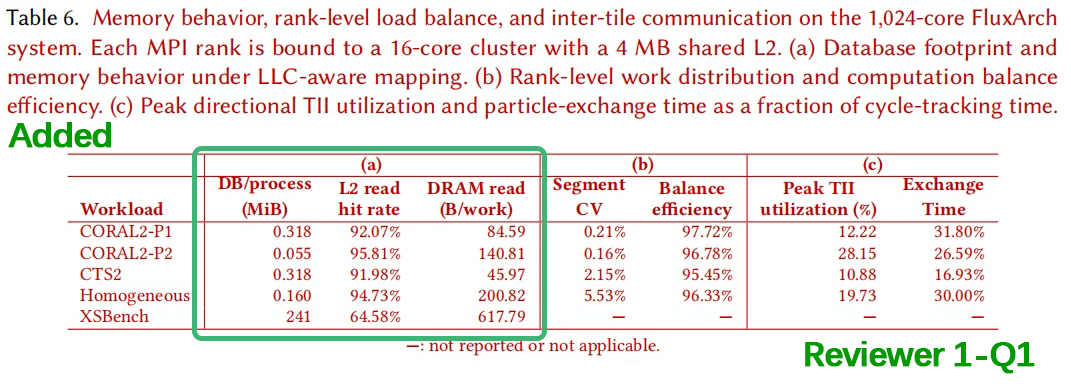
\includegraphics[width=0.9\textwidth]{news/R1-Q1-tab6a.png}}
\end{figure}
\end{minipage}\par\medskip

\end{enumerate}


\subsection{Question 2}
\begin{reviewcomment}
The thread affinity and spatial decomposition strategies described in Section 5 may introduce load imbalance, causing some cores to handle significantly more work than others. The authors acknowledge this as a limitation and suggest dynamic partitioning as a future work direction, but it would still be valuable to at least quantify the resulting imbalance and its impact on performance.
\end{reviewcomment}

Our static affinity and spatial decomposition assign one MPI rank to each cluster, so stochastic particle histories can create unequal work across the 64 ranks. We added a rank-level evaluation using both completed segments and accumulated tracking-kernel time rather than assuming perfect balance. The coefficient of variation (CV) of kernel time is only 1.17\%--2.01\%, balance efficiency is 95.45\%--97.72\%, and the resulting computation-side tail loss is at most 4.55\% for the evaluated inputs. These results indicate that static affinity and spatial decomposition maintain balanced computation across clusters for the evaluated workloads at 1,024 cores, with limited computation-side loss from load imbalance.

\revisionlocation{The rank-level load-balance method and its computation-side impact are evaluated in \textbf{Section 6.5}.}

\excerptlabel{Added (Section 6.5, pages 18--19):}\par
\begin{manuscriptexcerpt}
\redsentence{\textbf{Load Balance.}} \redsentence{Table~6(b) quantifies the concern that static affinity and spatial decomposition may assign unequal work to clusters.} \redsentence{We record completed segments and accumulated tracking-kernel time separately for all 64 ranks.} \redsentence{Segment-count CV ranges from 0.16\% to 5.53\%; because stochastic segments can follow different paths and incur different costs, count variation does not translate proportionally into execution-time variation.} \redsentence{Kernel-time CV remains 1.17\%--2.01\%.} \redsentence{We define balance efficiency as the mean rank-level kernel time divided by the maximum rank-level kernel time, since the slowest rank determines the computation tail.} \redsentence{The resulting efficiency is 95.45\%--97.72\%, corresponding to an estimated computation-side tail loss of at most 4.55\%.} \redsentence{These results indicate that static affinity and spatial decomposition maintain balanced computation across clusters for the evaluated workloads at 1,024 cores, with limited computation-side loss from load imbalance.}
\end{manuscriptexcerpt}
\par\noindent\begin{minipage}{\linewidth}
\revisionlocation{The segment-count variation and balance efficiency are added in \textbf{Table~6(b)}.}

\excerptlabel{Added (Table~6(b), page 18):}\par
% Revised manuscript: Table 6(b)
\begin{figure}[H]
  \centering
  \fbox{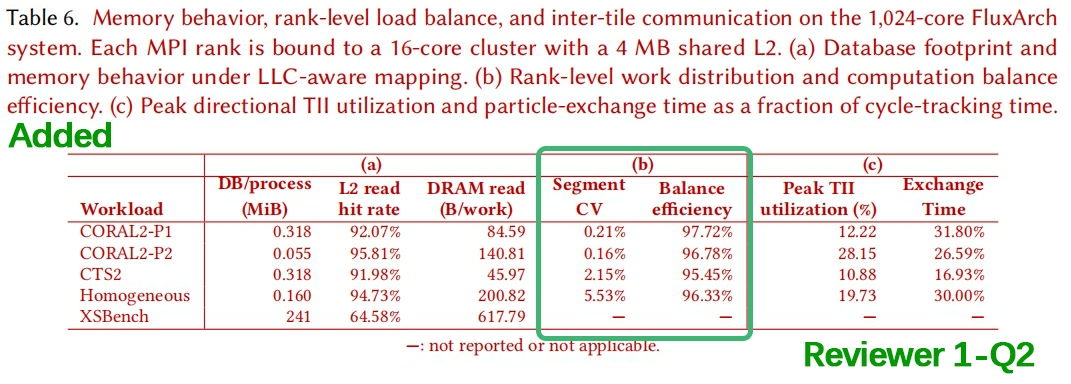
\includegraphics[width=0.9\textwidth]{news/R1-Q2-tab6b.png}}
\end{figure}
\end{minipage}\par\medskip

\subsection{Question 3}
\begin{reviewcomment}
A missing aspect of the experimental setup is the modeling of inter-tile communication. More details are needed to ensure reproducibility and properly contextualize the results.
\end{reviewcomment}

Inter-tile communication is explicitly modeled rather than treated as zero-cost functional transfer. We expanded the evaluation methodology to specify that MPI messages traverse the guest network stack, Intel Gigabit Ethernet (IGbE) endpoints, and \texttt{DistEtherLink}-based Tile Interconnection Interfaces (TIIs) and therefore incur protocol processing, packetization, serialization, and modeled link latency. We also added per-TII traffic and end-to-end particle-exchange measurements: the busiest direction reaches 10.88\%--28.15\% of the 1-Gb/s link capacity, while traffic CV across the eight TIIs is 0.50\%--2.42\%. Thus, communication has a measurable execution cost, but TII saturation or traffic imbalance is not the bottleneck in these experiments.

\revisionlocation{The MPI transport path and communication-cost measurement method are specified in \textbf{Section 6.1}.}

\excerptlabel{Added (Section 6.1, page 13):}\par
\begin{manuscriptexcerpt}
\redsentence{\textbf{Inter-Tile Communication Modeling.}} \redsentence{The eight Compute Tiles are connected to the Switch Tile through eight bidirectional Tile Interconnection Interfaces (TIIs).} \redsentence{In distributed full-system gem5, each TII is modeled using a \texttt{DistEtherLink} and an IGbE endpoint, with the directional 1-Gb/s capacity in Table~1 and the modeled inter-tile latency.} \redsentence{MPI messages traverse the guest network stack and these modeled links and are therefore subject to software protocol processing, packetization, link serialization, and inter-tile latency rather than zero-cost functional communication.} \redsentence{We use the Ethernet-device counters to measure transmitted bytes and directional utilization at every TII.} \redsentence{Quicksilver's cycle-tracking timers separately measure end-to-end particle-exchange time, including buffer handling, MPI communication and waiting, and receive-side particle management.}
\end{manuscriptexcerpt}
\revisionlocation{The measured TII utilization and traffic balance are analyzed in \textbf{Section 6.7}.}

\excerptlabel{Added (Section 6.7, page 21):}\par
\begin{manuscriptexcerpt}
\redsentence{Table~6(c) reports peak directional TII utilization and the particle-exchange share of cycle-tracking time.} \redsentence{Across CORAL2-P1, CORAL2-P2, CTS2 and Homogeneous, \name\ injects 1.37--1.46 bytes of inter-tile traffic per completed segment.} \redsentence{The busiest directional TII reaches only 10.88\%--28.15\% of its modeled 1-Gb/s capacity.} \redsentence{Bidirectional link traffic is also well balanced: its coefficient of variation across the eight TIIs is 0.50\%--2.42\%.} \redsentence{Thus, the communication-driven spatial mapping avoids TII hotspots, and the evaluated links remain below saturation.}
\end{manuscriptexcerpt}
\par\noindent\begin{minipage}{\linewidth}
\revisionlocation{The peak directional TII utilization and particle-exchange share are reported in \textbf{Table~6(c)}.}

\excerptlabel{Added (Table~6(c), page 18):}\par
% Revised manuscript: Table 6(c)
\begin{figure}[H]
  \centering
  \fbox{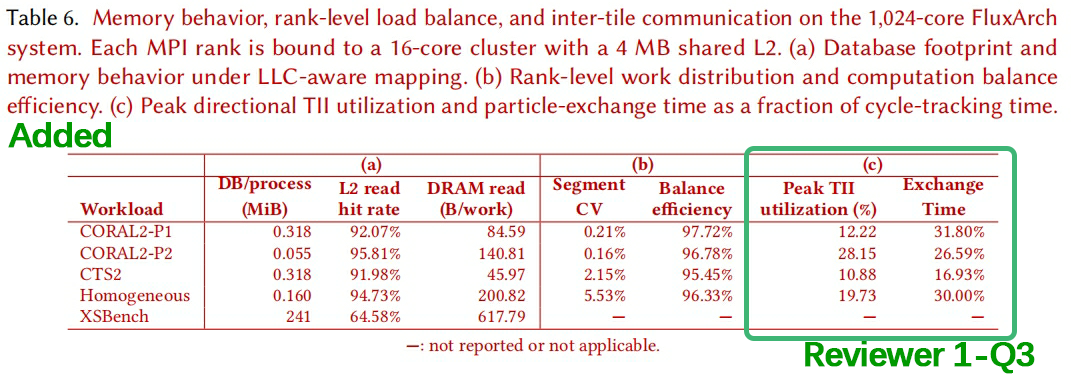
\includegraphics[width=0.9\textwidth]{news/R1-Q3-tab6c.png}}
\end{figure}
\end{minipage}\par\medskip


\subsection{Question 4}
\begin{reviewcomment}
In the experimental setup, there is no mention of random seed control or variability between runs, which are important details as MCPT is stochastic.
\end{reviewcomment}

We use the same fixed workload-default pseudorandom seed for each workload across platforms to support reproducibility. Each experiment is repeated 10 times under exclusive-platform and stable-thermal conditions, and we report the arithmetic mean of the workload-native performance metric. Across the platform--workload configurations in Figure~13(a), the throughput coefficient of variation (CV) ranges from 0.1\% to 6.2\%, and from 0.1\% to 0.4\% for \name. These values quantify run-to-run variability with the seed held fixed. We have added the repetition count and CV ranges to \textbf{Section 6.1}.

\revisionlocation{The seed policy and reporting of run-to-run variability are clarified in \textbf{Section 6.1}.}

\excerptlabel{Added (Section 6.1, page 14):}\par
\begin{manuscriptexcerpt}
\redsentence{\textbf{Reproducibility and Run-to-Run Variability}.} \redsentence{All platforms use fixed workload-default pseudorandom seeds (Table~\ref{tab:benchmarks}).} \redsentence{Each experiment is repeated 10 times, and we report the arithmetic mean of the workload-native performance metric.} \redsentence{Runs use exclusive platforms under stable thermal conditions.} \redsentence{For Fig.~13(a), the throughput coefficient of variation (CV) is 0.1\%--6.2\% across platform--workload configurations and 0.1\%--0.4\% for \name.}
\end{manuscriptexcerpt}

\par\noindent\begin{minipage}{\linewidth}
\revisionlocation{The workload seeds are specified in \textbf{Table~4}, which corresponds to \textbf{Table~2} in the original manuscript.}

\excerptlabel{Original (Table~2, page 14):}\par
% Original manuscript: Table 2
\begin{figure}[H]
  \centering
  \fbox{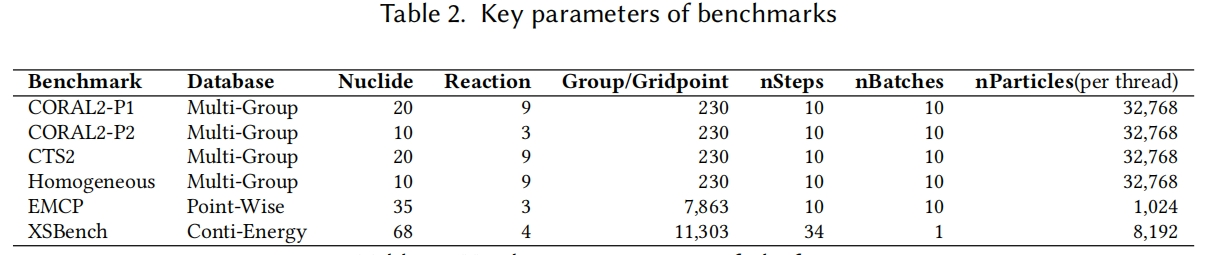
\includegraphics[width=0.9\textwidth]{figures/O-tab2.png}}
\end{figure}
\end{minipage}\par\medskip

\par\noindent\begin{minipage}{\linewidth}
\excerptlabel{Revised (Table~4, page 14):}\par
% Revised manuscript: Table 4
\begin{figure}[H]
  \centering
  \fbox{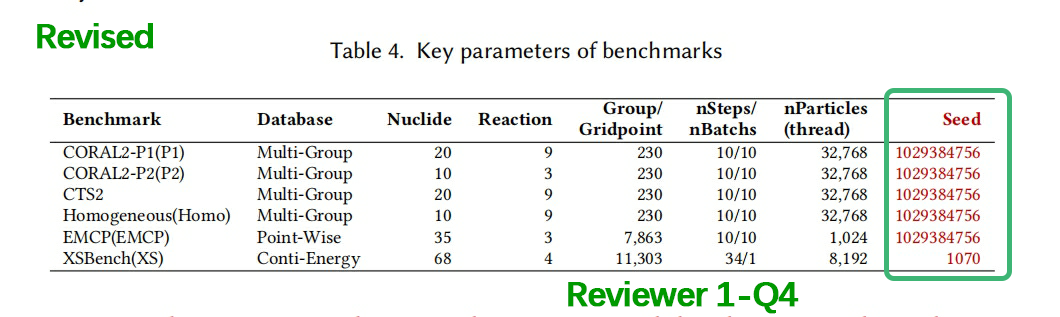
\includegraphics[width=0.9\textwidth]{news/R1-Q4-tab4.png}}
\end{figure}
\end{minipage}\par\medskip


\subsection{Question 5}
\begin{reviewcomment}
The authors describe how they measured the power for FluxArch but not for the baseline architectures. It is important to include such details for reproducibility and to ensure fair comparison (check the next cogent for the fairness).
\end{reviewcomment}

The CPU and GPU baselines run natively, whereas \name\ is evaluated through gem5 with McPAT and CACTI package-power modeling. We expanded the methodology to identify the measurement tools and align the accounting boundaries: \texttt{powerstat} records CPU/FT package power, \texttt{nvidia-smi} records GPU-board power, and off-package DDR5 is modeled separately where telemetry does not include it. This treatment includes co-packaged DDR4 or HBM only once and avoids omitting external DDR5 from the other platforms.

\revisionlocation{The native measurement tools, simulated power model, and measurement interval are specified in \textbf{Section 6.1}.}

\excerptlabel{Added (Section 6.1, page 14):}\par
\begin{manuscriptexcerpt}
\redsentence{\textbf{Power and Area Modeling Methodology}.} \redsentence{Table~5(b) distinguishes the measured and simulated platforms and defines the power-accounting boundary.} \redsentence{We execute all baselines natively.} \redsentence{For \intel, \amd, and \ft, we collect on-package power with \texttt{powerstat}~\papercite{powerstat}; for \ampare\ and \hopper, we record GPU-board power with \texttt{nvidia-smi}~\papercite{nvidia_smi}.} \redsentence{We report the mean power observed during each workload's timed execution region.} \redsentence{\name\ is evaluated in gem5, with package power modeled using McPAT and CACTI.}
\end{manuscriptexcerpt}
\begin{excerptreferences}
\paperreference{powerstat}
\paperreference{nvidia_smi}
\end{excerptreferences}

\par\noindent\begin{minipage}{\linewidth}
\revisionlocation{The platform-specific measurement and power-accounting boundaries are clarified in \textbf{Table~5}, which corresponds to original \textbf{Table~3}. Panel (a) revises the platform specifications, while panel (b) adds the evaluation methods and power-accounting boundaries.}

\excerptlabel{Original (Table~3, page 14):}\par
% Original manuscript: Table 3
\begin{figure}[H]
  \centering
  \fbox{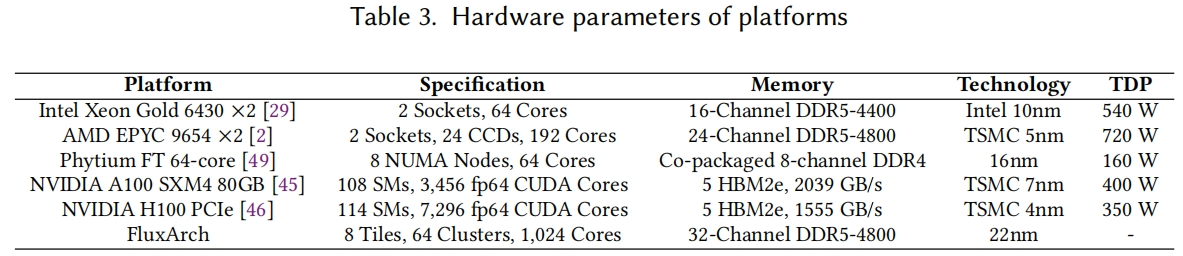
\includegraphics[width=0.9\textwidth]{figures/O-tab3.png}}
\end{figure}
\end{minipage}\par\medskip

\par\noindent\begin{minipage}{\linewidth}
\excerptlabel{Revised (Table~5, page 15):}\par
% Revised manuscript: Table 5
\begin{figure}[H]
  \centering
  \fbox{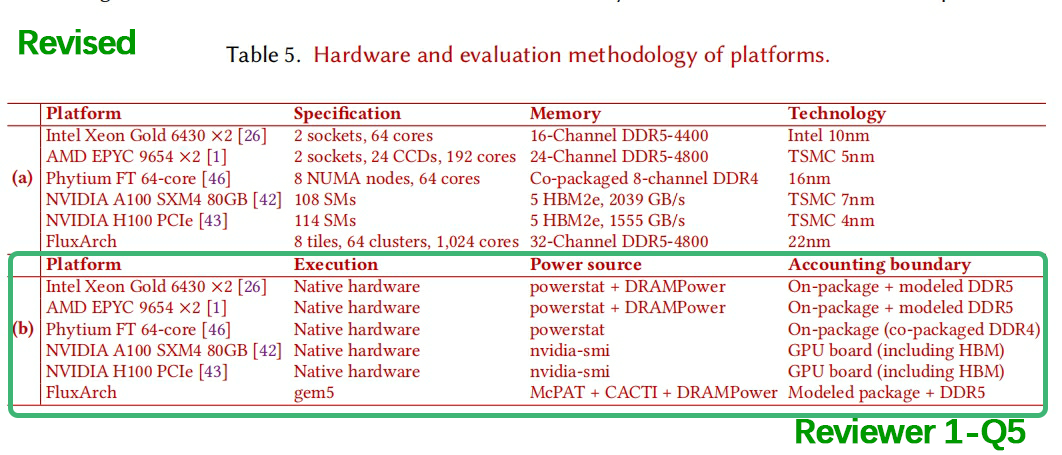
\includegraphics[width=0.9\textwidth]{news/R1-Q5-tab5.png}}
\end{figure}
\end{minipage}\par\medskip

\subsection{Question 6}
\begin{reviewcomment}
The authors mention that all reported energy metrics focus exclusively on on-chip power and that off-chip DRAM power is excluded. However, this makes the energy comparisons not very informative and, in cases, unfair. This is especially the case when comparing against architectures that have L3 cache. As FluxArch has no shared L3 cache, it is likely to have more misses than the baselines with L3 cache. Moreover, the baselines with L3 cache get unfairly penalized as their L3 power is included.
\end{reviewcomment}

We agree that on-chip-only energy accounting can bias a memory-bound comparison, especially when the platforms expose different memory-packaging boundaries. We therefore changed the evaluation to include co-packaged DDR4/HBM through device telemetry and off-package DDR5 through a common traffic-based DRAMPower~\papercite{drampower} model, with a $0.5\times$--$2\times$ sensitivity range for the modeled component. After this correction, the conservative process-scaled geometric-mean DRAM-inclusive energy-efficiency advantage remains 1.77$\times$ over H100 and 6.65$\times$ over Intel.

We now explain the choice of the $0.5\times$--$2\times$ range in \textbf{Section 6.1}. Ghose et al.~\papercite{ghose2018vampire} measured DDR3L read currents averaging 54.1\% below datasheet values for one vendor and data-pattern-dependent read-power differences of up to 91.6\%. Shi et al.~\papercite{shi2025drampower} report that DDR4 calibration reduced DRAMPower energy estimates by roughly half for most evaluated SPEC2006 workloads. These results motivate testing sizable modeling discrepancies, but do not establish an error bound for our DDR5 configuration. We therefore select reciprocal factors of 0.5 and 2 to test both overestimation and underestimation, with package power fixed; the range is a sensitivity-analysis choice, not a statistical confidence interval.

For process-scaled energy-efficiency bounds, we independently vary only the scaled FluxArch package power by $\pm30\%$ and each modeled off-package DRAM component over $0.5\times$--$2\times$, while keeping throughput and measured baseline package power fixed. We recompute the performance/W ratio at every endpoint combination and report its minimum and maximum; external DRAM power is not subject to process-node scaling or its 30\% margin.


\revisionlocation{The power-accounting boundary is revised in \textbf{Section 6.1} to include DRAM consistently across platforms.}

\excerptlabel{Revised (Section 6.1, page 14):}\par
\begin{manuscriptexcerpt}
\redsentence{We report DRAM-inclusive system power and energy.} \redsentence{Package power includes cores, caches, NoCs, and integrated memory controllers; for \ft, \ampare, and \hopper, the main memory is co-packaged (DDR4 or HBM) and is consequently covered by platform-level package/device telemetry.} \redsentence{In contrast, the DDR5 DIMMs of \intel\ and \amd, and the DDR5 channels assumed for \name, are physically off-package and are not covered by package-power readings.} \redsentence{We therefore add a separately modeled DRAM component to these platforms, avoiding asymmetric accounting that would include HBM/DDR4 power for the co-packaged-memory platforms but omit DDR5 power for the other platforms.}

\end{manuscriptexcerpt}

\revisionlocation{The traffic-based DRAM model and factor-of-two sensitivity analysis are added in \textbf{Section 6.1}.}

\excerptlabel{Added (Section 6.1, pages 14--15):}\par
\begin{manuscriptexcerpt}
\redsentence{For the DRAM model, we use DRAMPower 5~\papercite{drampower} with DDR5 timing and worst-case current parameters from the JEDEC DDR5 standard~\papercite{jedec_ddr5} and the Micron MT60B2G8HB-48B DDR5-4800 x8 datasheet~\papercite{micron_ddr5}.} \redsentence{\name\ is modeled with 32 single-rank DDR5-4800 channels, each containing eight x8 DRAM devices.} \redsentence{The model includes active-standby background power, refresh power, and read/write transfer power.} \redsentence{The external-memory energy of \intel\ and \amd\ is estimated using the same traffic-based DDR5 model and workload-specific memory traffic.}

\redsentence{Because the simulation does not expose DRAM command traces or row-buffer events, we use a traffic-based DRAM energy estimate rather than claiming command-level precision.} \redsentence{For each \name\ workload, we derive read/write traffic from the memory-system statistics and use the simulated execution time.} \redsentence{Prior DRAM measurement and calibration studies report substantial discrepancies between datasheet-based estimates and measured consumption~\papercite{ghose2018vampire,shi2025drampower}.} \redsentence{Motivated by these findings, we select a $0.5\times$--$2\times$ range for the nominal modeled DRAM power of every off-package DDR5 platform (\intel, \amd, and \name).} \redsentence{This range is a sensitivity-analysis choice, not an empirically established DDR5 error bound or a statistical confidence interval.}
\end{manuscriptexcerpt}
\begin{excerptreferences}
\paperreference{drampower}
\paperreference{jedec_ddr5}
\paperreference{micron_ddr5}
\paperreference{ghose2018vampire}
\paperreference{shi2025drampower}
\end{excerptreferences}

\revisionlocation{The energy-efficiency comparison and conservative lower bounds are updated in \textbf{Section 6.2} to include DRAM power.}

\excerptlabel{Original (Section 6.2, pages 14--15):}\par
\begin{manuscriptexcerpt}
\graysentence{\textbf{Iso-Process Energy Efficiency}.} \graysentence{As shown in Fig.~13(b), the energy efficiency advantage is even more pronounced.} \graysentence{By comparing projected iso-process nodes, we isolate the architectural contributions.} \graysentence{According to Section. 6.1, the power projection error is 30\%.} \graysentence{Therefore, we incorporate this margin into our energy efficiency evaluation, which is represented as error bars in our results.} \graysentence{Without the workload orchestration, the energy efficiency of \name, mainstream server CPUs and high-end GPUs is at odds with each other.} \graysentence{With the orchestration enabled, optimizing data locality and minimizing cross-tile traffic, \name\ demonstrates a superior geometric mean energy efficiency improvement from \textbf{3.98}$\boldsymbol{\times}$ (vs. \ft, 5.69$\times$ discounted by 30\%) to \textbf{9.84}$\boldsymbol{\times}$ (vs. \intel, 14.06$\times$ discounted by 30\%) even accounting for the potential projection error of pessimistic assumption.} \graysentence{We also report the energy efficiency of the raw, unscaled data based on the 22 nm technology node.} \graysentence{Even in this case, \name\ still achieves an energy efficiency improvement of 1.17$\times$ (vs. \hopper) to 4.59$\times$ (vs. \intel).}
\end{manuscriptexcerpt}

\excerptlabel{Revised (Section 6.2, pages 15--16):}\par
\begin{manuscriptexcerpt}
\redsentence{\textbf{DRAM-Inclusive Energy Efficiency}.} \redsentence{Fig.~13(c,d) reports DRAM-inclusive power and energy efficiency under the sensitivity bounds defined in Section 6.1.} \redsentence{Process-scaled results separate architectural effects from process scaling while accounting consistently for external memory.}

\redsentence{In the process-scaled comparison, \name\ improves geometric-mean DRAM-inclusive efficiency by \textbf{2.85}$\boldsymbol{\times}$ over \hopper\ to \textbf{10.58}$\boldsymbol{\times}$ over \intel.}

\redsentence{The sensitivity analysis preserves the process-scaled conclusion: across the combined DRAM and technology-scaling bounds, the geometric-mean improvement with orchestration remains 1.77$\times$ over \hopper\ and 6.65$\times$ over \intel\ at the conservative lower bound.}

\end{manuscriptexcerpt}

\par\noindent\begin{minipage}{\linewidth}
\revisionlocation{The power breakdown and energy-efficiency plots are updated in \textbf{Figure~13(c,d)} to include DRAM power and the corresponding sensitivity bounds. Panel (c) is newly added; panel (d) revises the original energy-efficiency plot.}

\excerptlabel{Original (Figure~13, page 15):}\par
% Original manuscript: Figure 13
\begin{figure}[H]
  \centering
  \fbox{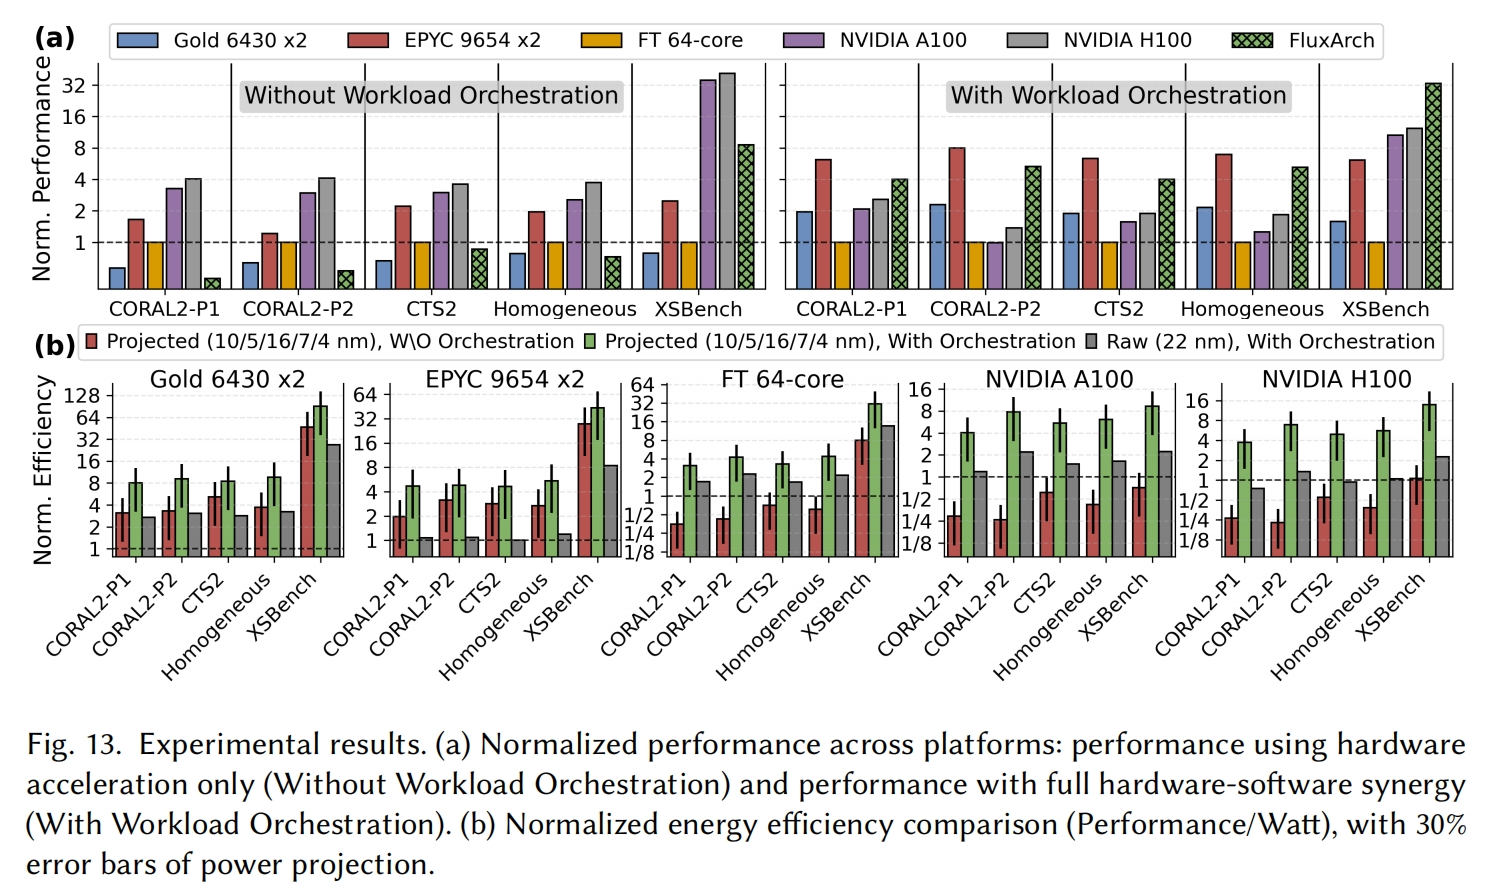
\includegraphics[width=0.9\textwidth]{figures/O-fig13.png}}
\end{figure}
\end{minipage}\par\medskip

\par\noindent\begin{minipage}{\linewidth}
\excerptlabel{Revised (Figure~13, page 16):}\par
% Revised manuscript: Figure 13
\begin{figure}[H]
  \centering
  \fbox{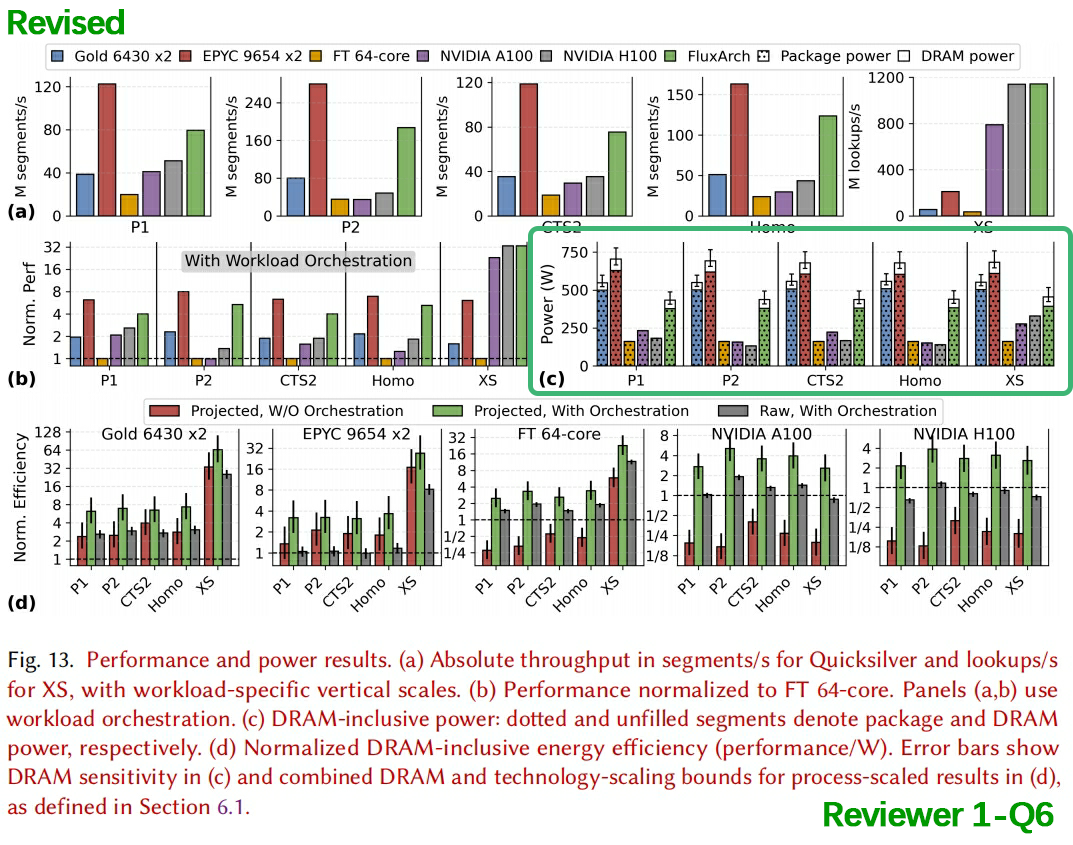
\includegraphics[width=0.9\textwidth]{news/R1-Q6-fig13.png}}
\end{figure}
\end{minipage}\par\medskip


\subsection{Question 7}
\begin{reviewcomment}
In Section 6.6 on scalability evaluation, the authors argue that the Gold 6430 $\times$2 and FT 64-core outperform the proposed approach because their monolithic LLCs provide a unified, low-latency shared memory space that enables efficient inter-thread synchronization at lower core counts. However, no empirical data is provided to support this claim. Do the authors have measurements or analysis validating this explanation? This is particularly important since both systems significantly outperform FluxArch in most cases, and no experiments beyond 64 cores are possible to demonstrate whether FluxArch would eventually surpass them at larger scales (as they have no more cores).
\end{reviewcomment}

We do not have controlled measurements that isolate LLC organization as the cause of the observed scaling difference. Cache organization, memory hierarchy, core microarchitecture, and synchronization overhead vary together across the evaluated platforms. The commercial baseline systems expose tightly coupled hardware configurations that cannot be independently reconfigured to change only LLC organization while holding the other factors constant. Our measurements therefore do not support the earlier LLC-based causal explanation, which we have removed. The revised discussion reports only the observed scaling trends within the evaluated ranges, without extrapolating Intel or FT beyond 64 cores.


\revisionlocation{The scaling discussion is revised in \textbf{Section 6.6} to distinguish the measured trends from an unisolated LLC-based explanation and limit the CPU comparison to the evaluated range.}

\excerptlabel{Original (Section 6.6, page 17):}\par
\begin{manuscriptexcerpt}
\graysentence{Fig.~17 evaluates the scaling efficiency of \name\ against three CPU platforms.} \graysentence{In the small-scale regime ($<64$ cores), \name\ and \amd\ exhibit low efficiency.} \graysentence{This is attributed to the architectural trade-off between monolithic and distributed Last-Level Caches (LLCs).} \graysentence{Monolithic LLCs (\intel/\ft) provide a unified, low-latency shared memory pool that excels at handling inter-thread synchronization with a low core count.} \graysentence{Conversely, the distributed LLCs in \name\ and \amd\ incur higher coherence overhead when the workload is concentrated in fewer cores, as the shared memory programming model imposes a latency barrier on cross-cluster communication.} \graysentence{However, in the large-scale regime ($>64$ cores), \name's hierarchical design demonstrates superior efficiency, surpassing \amd\ across nearly all benchmarks as the system scales.}
\end{manuscriptexcerpt}

\excerptlabel{Revised (Section 6.6, page 20):}\par
\begin{manuscriptexcerpt}
\redsentence{\textbf{System-Level Scalability.}} \redsentence{Fig.~18 evaluates the scaling efficiency of \name\ against three CPU platforms.} \redsentence{At up to 64 cores, \intel\ and \ft\ retain higher scaling efficiency than \name\ for most workloads.} \redsentence{Cache organization, memory hierarchy, core microarchitecture, and synchronization overhead vary jointly across these platforms.} \redsentence{The commercial baselines do not provide otherwise identical configurations differing only in LLC organization, so this cross-platform comparison characterizes system-level scaling rather than the isolated effect of LLC design.} \redsentence{The evaluated \intel\ and \ft\ configurations cover at most 64 cores, limiting the comparison to this range.} \redsentence{Within the measured range, \name\ continues scaling to 1,024 cores and exceeds the measured \amd\ scaling efficiency across nearly all workloads at larger core counts.}
\end{manuscriptexcerpt}

\par\noindent\begin{minipage}{\linewidth}
\excerptlabel{Figure~18 (page 20):}\par
% Manuscript: Figure 18
\begin{figure}[H]
  \centering
  \fbox{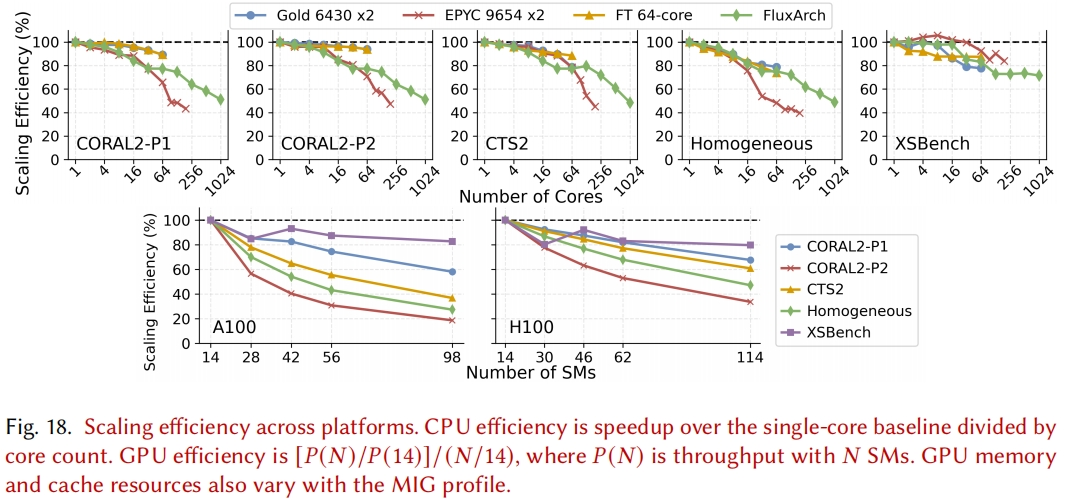
\includegraphics[width=0.9\textwidth]{figures/fig18.png}}
\end{figure}
\end{minipage}\par\medskip


\subsection{Question 8}
\begin{reviewcomment}
Why are no scalability results presented for GPUs? There are different ways to limit the GPU usage and emulate scalability. The authors are recommended to add such results or provide good reasons not to.
\end{reviewcomment}

We added GPU scaling measurements by fixing each workload's problem size and increasing the number of streaming multiprocessors (SMs) assigned to one GPU instance through NVIDIA Multi-Instance GPU (MIG). The five profiles provide 14, 28, 42, 56, and 98 SMs on A100, and 14, 30, 46, 62, and 114 SMs on H100. Each workload runs on one instance at a time. Efficiency is $E(N)=[P(N)/P(14)]/(N/14)$, where $P(N)$ is throughput with $N$ SMs. Because memory capacity, cache, and memory bandwidth also depend on the profile, these results characterize scaling across GPU resource configurations. At 98 SMs on A100 and 114 SMs on H100, efficiency ranges from 18.62\% to 82.73\% and from 33.65\% to 79.65\%, respectively; XSBench scales best and CORAL2-P2 scales least efficiently on both GPUs.

\revisionlocation{The MIG allocation method, normalization, and GPU scaling trends are described in \textbf{Section 6.6}.}

\excerptlabel{Added (Section 6.6, page 20):}\par
\begin{manuscriptexcerpt}
\redsentence{We additionally evaluate GPU scaling by keeping each workload's problem size fixed and increasing the number of streaming multiprocessors (SMs) assigned to one GPU instance. NVIDIA Multi-Instance GPU (MIG) partitions a physical GPU into isolated instances with dedicated compute and memory resources. We use five MIG profiles to allocate 14--98 SMs on \ampare, and 14--114 SMs on \hopper. The cache and memory-bandwidth allocations vary with the profile, so these measurements reflect scaling across GPU resource configurations. At 98 SMs on \ampare\ and 114 SMs on \hopper, efficiency ranges from 18.62\% to 82.73\% and from 33.65\% to 79.65\%, respectively. XSBench scales best on both GPUs, while CORAL2-P2 scales least efficiently.}
\end{manuscriptexcerpt}

\par\noindent\begin{minipage}{\linewidth}
\revisionlocation{The GPU scaling results are added in \textbf{Figure~18}, with GPU scale labeled by the actual SM counts. The CPU panels are revised from the original figure, while the GPU panels are newly added.}

\excerptlabel{Revised (Figure~18, page 20):}\par
% Revised manuscript: Figure 18
\begin{figure}[H]
  \centering
  \fbox{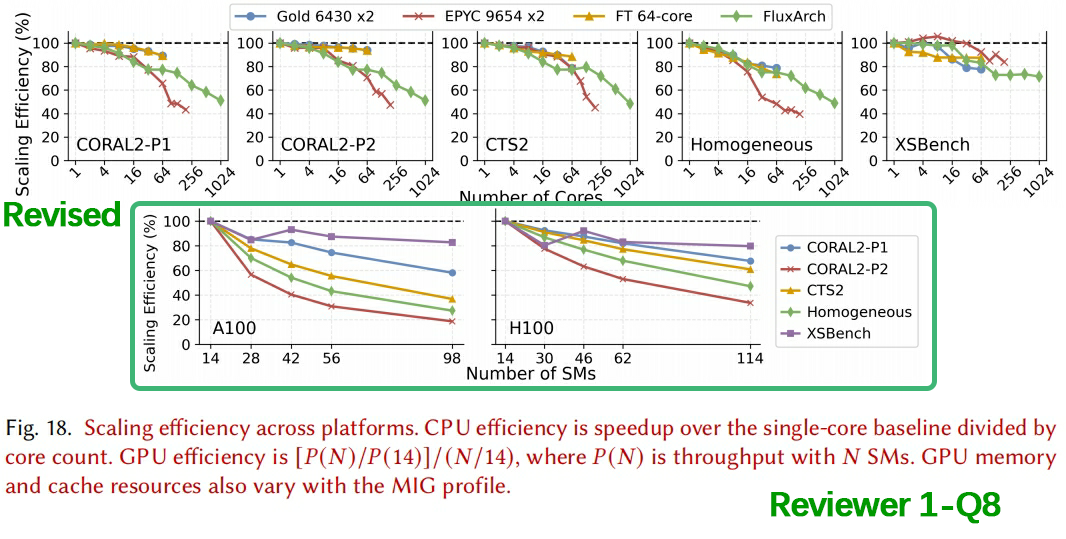
\includegraphics[width=0.9\textwidth]{news/R1-Q8-fig18.png}}
\end{figure}
\end{minipage}\par\medskip

\subsection{Question 9}
\begin{reviewcomment}
The scalability behaviour of the XSBench benchmark is an outlier. The authors are recommended to discuss the reason behind this. Are there certain generalizable characteristics in this benchmark that affect FluxArch and EPYC scaling?
\end{reviewcomment}

We revised \textbf{Figure~18} for clarity and aligned the y-axis scales across panels.

XSBench is an outlier in the favorable direction: it retains approximately 71\% scaling efficiency at 1,024 cores, compared with approximately 48\%--52\% for the other \name\ workloads. On EPYC, XSBench similarly retains approximately 84\% efficiency at 192 cores, compared with approximately 40\%--47\% for the four Quicksilver workloads. EPYC and \name\ both organize cores into local cache-sharing groups---CCDs sharing L3 and clusters sharing L2, respectively. Under our LLC-aware process mapping, XSBench's independent lookups require no inter-rank particle-state exchange as execution expands across these groups, unlike Quicksilver. This favorable scaling does not imply full cache residency: its 241-MiB database exceeds the 4-MiB cluster L2 on \name, and the \name\ measurements in Table~6(a) report the lowest L2 read hit rate and highest normalized DRAM read traffic among the evaluated workloads. We clarified this shared workload characteristic and its relationship to the two platforms' cache-sharing groups in \textbf{Section 6.6}.


\par\noindent\begin{minipage}{\linewidth}
\excerptlabel{Original (Figure~17, page 18):}\par
% Original manuscript: Figure 17
\begin{figure}[H]
  \centering
  \fbox{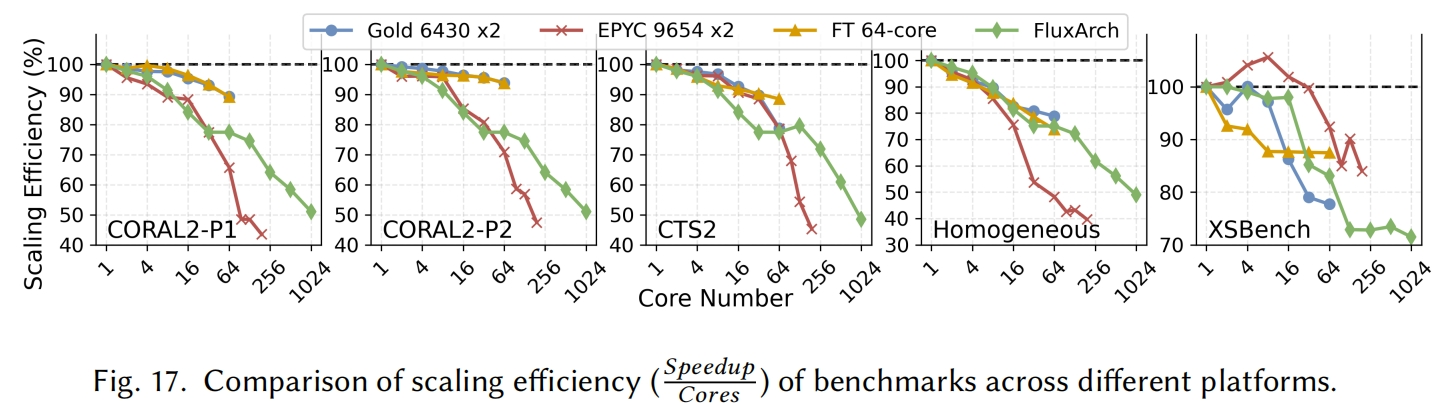
\includegraphics[width=0.9\textwidth]{figures/O-fig17.png}}
\end{figure}
\end{minipage}\par\medskip

\par\noindent\begin{minipage}{\linewidth}
\excerptlabel{Revised (Figure~18, page 20):}\par
% Revised manuscript: Figure 18
\begin{figure}[H]
  \centering
  \fbox{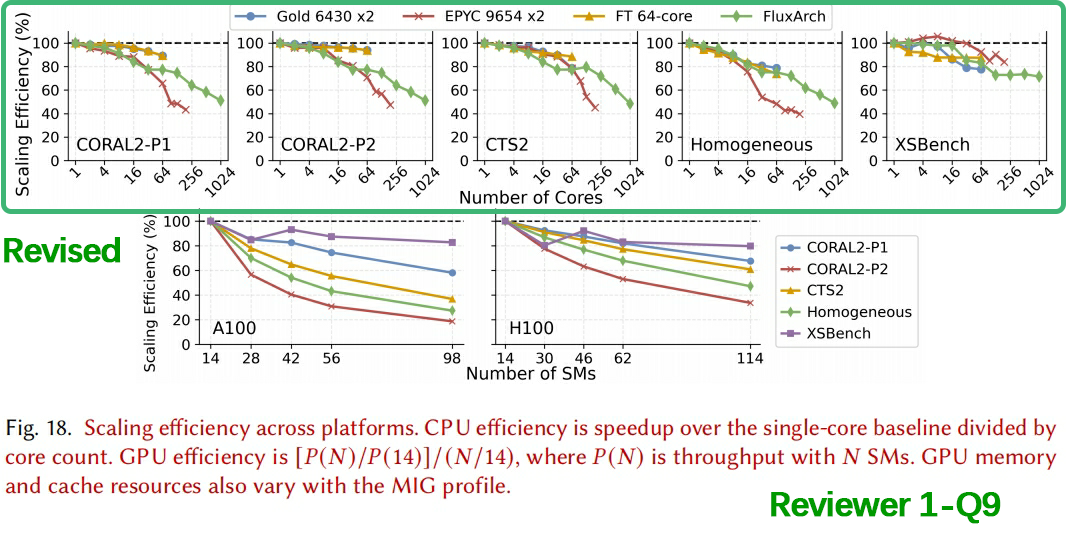
\includegraphics[width=0.9\textwidth]{news/R1-Q9-fig18.png}}
\end{figure}
\end{minipage}\par\medskip



\revisionlocation{The favorable XSBench scaling is explained in \textbf{Section 6.6} through its independent lookups and absence of inter-rank particle exchange.}

\excerptlabel{Added (Section 6.6, page 20):}\par
\begin{manuscriptexcerpt}
\redsentence{XSBench retains approximately 71\% scaling efficiency at 1,024 cores, compared with approximately 48\%--52\% for the other \name\ workloads.} \redsentence{EPYC and \name\ both organize cores into local cache-sharing groups---CCDs sharing L3 and clusters sharing L2, respectively.} \redsentence{Under our LLC-aware process mapping, XSBench's independent lookups require no inter-rank particle-state exchange as execution expands across these groups, unlike Quicksilver.} \redsentence{This favorable scaling does not imply full cache residency: the \name\ measurements in Table~6(a) show that XSBench has the largest database, the lowest L2 read hit rate, and the highest normalized DRAM read traffic among the evaluated workloads.}
\end{manuscriptexcerpt}

\revisionlocation{The discussion also relates this behavior to the memory measurements in \textbf{Table~6(a)}.}
\par\noindent\begin{minipage}{\linewidth}
\excerptlabel{Added (Table~6(a), page 18):}\par
% Revised manuscript: Figure 6(a)
\begin{figure}[H]
  \centering
  \fbox{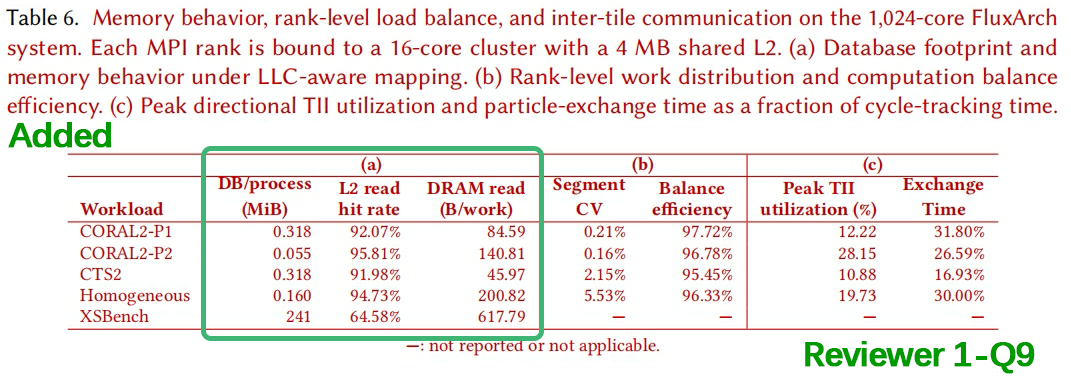
\includegraphics[width=0.9\textwidth]{news/R1-Q9-tab6a.png}}
\end{figure}
\end{minipage}\par\medskip

\subsection{Question 10}
\begin{reviewcomment}
The authors primarily evaluate CPUs and GPUs, but do not discuss alternative architectures such as FPGAs, CGRAs, or specialized manycore systems like Graphcore. These platforms may help mitigate some of the bottlenecks identified for CPUs and GPUs. In addition, prior work has explored FPGA-based approaches for Monte Carlo simulations. A comparison (discussion, not necessarily a complete evaluation) would strengthen the paper and provide a more complete perspective on the proposed architecture's position in the design space.
\end{reviewcomment}

We agree that FPGA-based Monte Carlo transport acceleration is relevant prior work and was insufficiently discussed in the original manuscript. We now explicitly discuss Gokhale et al.'s FPGA pipeline for ray--surface intersection in Monte Carlo radiative heat transfer and Luu et al.'s FPGA implementation of MCML photon transport. The comparison in \textbf{Section 8} is anchored in the boundary of specialization: these works specialize a transport loop or a particular photon-transport pipeline, whereas \name\ retains instruction-driven MIMD transport control and integrates selected FP64 arithmetic kernels into each core. Their application-specific datapaths do not establish the cache/DRAM and communication organization used here for database-intensive neutron transport. We explain how \name\ combines core-local acceleration with shared-cache reuse and topology-aware MPI/OpenMP orchestration, rather than suggesting that FPGAs cannot handle stochastic control. We also distinguish CGRA spatial mapping from instruction-driven control and Graphcore's tile-local memory/exchange organization from \name's cache/DRAM hierarchy. The discussion compares design choices, not speedup values obtained under different physical models and workloads.

\revisionlocation{The architectural differences from FPGAs, CGRAs, and the Graphcore IPU, together with the limits of a quantitative comparison, are clarified in \textbf{Section 8}.}

\excerptlabel{Added (Section 8, pages 22--23):}\par
\begin{manuscriptexcerpt}
\redsentence{\textbf{Alternative Programmable Architectures.}} \redsentence{Gokhale et al.~\papercite{gokhale2004radiative} accelerate Monte Carlo radiative heat transfer with an FPGA ray--surface intersection pipeline; Luu et al.~\papercite{luu2009mcml} implement MCML photon transport through multilayer tissue as a dedicated FPGA pipeline.} \redsentence{The distinction is the boundary of specialization: these designs specialize a transport loop or photon-transport pipeline, whereas \name\ retains instruction-driven MIMD transport control and specializes selected FP64 arithmetic kernels within each core.} \redsentence{Their datapaths target the geometry and interaction models of their respective applications.} \redsentence{\name\ couples its core-local Engines with cache- and DRAM-backed database access and topology-aware MPI/OpenMP orchestration, addressing data reuse and inter-process communication alongside arithmetic acceleration.} \redsentence{CGRAs likewise expose configurable spatial datapaths, with computation mapped onto processing elements and their interconnect~\papercite{cgra-survey}; \name\ instead leaves dynamic transport control in programmable cores.} \redsentence{The Graphcore IPU is also MIMD, but its tile-local memory and explicit exchange~\papercite{ipu-particle-physics} contrast with \name's cache/DRAM hierarchy and core-local Engine.} \redsentence{Differences in physical models, workloads, and evaluation conditions preclude a direct comparison of the cited speedup values.}
\end{manuscriptexcerpt}
\begin{excerptreferences}
\paperreference{gokhale2004radiative}
\paperreference{luu2009mcml}
\paperreference{cgra-survey}
\paperreference{ipu-particle-physics}
\end{excerptreferences}

\subsection{Question 11}
\begin{reviewcomment}
The authors mentioned related architectures are using specialized, area-efficient designs (Fu et al [22] and Zhang et al. [72]). However, there is no comparison with these approaches. In the related work section, the authors mention briefly how FluxArch qualitatively improves over these works but do not provide any quantitative comparisons. The authors are recommended to include a more detailed comparison against the mentioned approaches as this would strengthen the work considerably.
\end{reviewcomment}

Fu et al. and Zhang et al. propose the specialized MCPT architectures most closely related to \name. We added a detailed comparison in \textbf{Table~7}, covering core design, hierarchy and system scale, cache and memory organization, evaluation methodology, workloads, and the quantitative results reported by each work.

We also explain in \textbf{Section 8} why these published values cannot be compared directly. Fu et al. report performance, performance/W, and performance/area relative to a modeled four-core Cortex-A15 system; Zhang et al. report scaling efficiency relative to their own single-core configuration. \name's performance and energy-efficiency ratios instead use our CPU/GPU baselines. Workload inputs, system resources, and accounting boundaries also differ substantially. The table therefore preserves each result's original baseline rather than converting these values into cross-architecture speedups.

Reimplementing the designs in a common framework would not, by itself, establish a fair comparison. Although the papers provide major architectural parameters, their descriptions do not fully specify all implementation and modeling choices needed for a unified evaluation. In particular, Zhang et al. do not report a process node or a power/area model. Reconstructing customized simulator configurations and adding missing power/area models would require assumptions that could affect the results and confound architectural differences with reconstruction choices.

\revisionlocation{The comparison with Fu et al. and Zhang et al. is revised in \textbf{Section 8} to clarify the architectural differences.}

\excerptlabel{Original (Section 8, page 19):}\par
\begin{manuscriptexcerpt}
\graysentence{Recent microarchitectural studies have shifted toward specialized, area-efficient designs.} \graysentence{Fu et al. pioneered the use of clustered small cores to improve energy-to-area ratios for MCPT workloads, a foundation subsequently extended by Zhang et al. to a 128-core cluster with optimized parallelization.} \graysentence{Our \name\ system achieves a significant leap forward by: (1) scaling the architecture to 1,024 cores using a hierarchical chiplet-based design; (2) integrating a dedicated execution engine to offload dominant kernels; and (3) proposing a topology-aware hardware-software co-design that transcends the scalability limits of prior clustered small-core architectures.}
\end{manuscriptexcerpt}

\excerptlabel{Revised (Section 8, page 22):}\par
\begin{manuscriptexcerpt}
\redsentence{\textbf{Specialized MCPT Architectures.}} \graysentence{Recent microarchitectural studies have shifted toward specialized, area-efficient designs.} \redsentence{Table~7 compares \name\ with Fu et al.~\papercite{minimctad} and Zhang et al.~\papercite{128mc} in core design, hierarchy, cache and memory organization, evaluation methodology, workloads, and author-reported results.} \redsentence{Fu et al. use simplified in-order cores to improve area and power efficiency, while Zhang et al. scale to 128 cores through 32-core cache-sharing clusters and OpenMP dynamic scheduling.} \redsentence{\name\ combines a 1,024-core hierarchy with a core-local Engine and topology-aware spatial mapping.}

\end{manuscriptexcerpt}
\begin{excerptreferences}
\paperreference{minimctad}
\paperreference{128mc}
\end{excerptreferences}

\revisionlocation{The limits of comparing published results and reconstructing prior designs fairly are added in \textbf{Section 8}.}

\excerptlabel{Added (Section 8, page 22):}\par
\begin{manuscriptexcerpt}
\redsentence{The reported results use substantially different experimental conditions, including workload inputs, core counts, cache and memory configurations, reference baselines, and power-accounting boundaries.} \redsentence{Fu et al. report performance, performance/W, and performance/area relative to a modeled four-core Cortex-A15 system.} \redsentence{Zhang et al. report scaling efficiency relative to their own single-core configuration.} \redsentence{\name's performance and energy-efficiency ratios use the evaluated CPU/GPU platforms as baselines, whereas its scaling efficiency is relative to one core.} \redsentence{Thus, Table~7 places each work's results in context rather than establishing cross-architecture speedups or an efficiency ranking.}

\redsentence{A unified reimplementation would also require resolving implementation and modeling choices not fully specified in the papers, rather than merely matching their listed hardware parameters.} \redsentence{In particular, Zhang et al. do not report a process node or a power/area model.} \redsentence{Reconstructing the customized simulator configurations and supplying missing power/area models would introduce additional assumptions that could affect the results, confounding architectural differences with reconstruction choices and weakening the fairness of a direct comparison.}


\end{manuscriptexcerpt}


\par\noindent\begin{minipage}{\linewidth}
\revisionlocation{The detailed architectural parameters and author-reported results, with their original comparison baselines, are added in \textbf{Table~7}.}

\excerptlabel{Added (Table~7, page 22):}\par
% Revised manuscript: Table 7
\begin{figure}[H]
  \centering
  \fbox{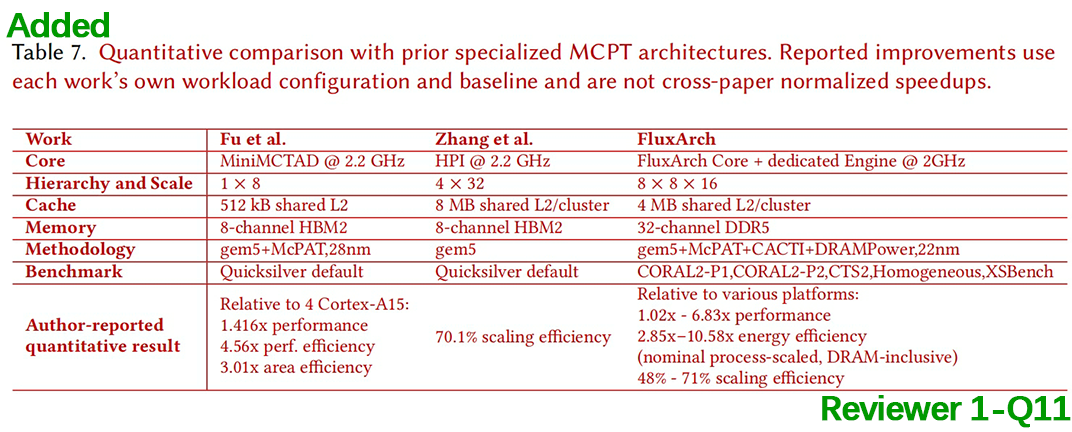
\includegraphics[width=0.9\textwidth]{news/R1-Q11-tab7.png}}
\end{figure}
\end{minipage}\par\medskip

\subsection{Question 12}
\begin{reviewcomment}
The authors are recommended to add references to the first paragraphs of the introduction for readers interested in more details.
\end{reviewcomment}

We sincerely thank you for your helpful and constructive suggestion. We added the corresponding references.


\revisionlocation{References supporting the introductory motivation and background claims are added in \textbf{Section 1}.}

\excerptlabel{Original (Section 1, page 1):}\par
\begin{manuscriptexcerpt}
\graysentence{Monte Carlo Particle Transport (MCPT) is the authoritative standard for simulating interactions between particles and material, widely applied in critical fields such as nuclear reactor safety and medical radiation therapy.} \graysentence{Its core philosophy involves performing independent and repeated random simulations of billions of particles and estimating macroscopic physical quantities, such as particle penetration probability and energy deposition distribution, based on statistical methods.} \graysentence{Since each particle is statistically independent, MCPT theoretically possesses rich parallel potential.}

\graysentence{However, in practice, each particle's transport is driven by random sampling, which determines its energy state, reaction type (e.g., fission, capture), and interaction position via probability distributions.} \graysentence{This stochastic nature renders particle execution paths highly unpredictable, thereby introducing extensive random control flow.} \graysentence{As particles propagate, they must frequently access multi-dimensional probability databases based on their current energy and reaction states to perform interpolation and physical calculations.} \graysentence{Since particles traverse highly dissimilar energy regions in state space, successive steps often access widely separated entries in the probability tables, resulting in significant spatial irregularity in memory access.}

\graysentence{Consequently, the MCPT workload simultaneously exhibits Massive Parallelism, Random Control Flow, and Irregular Memory Access---a combination of characteristics that poses extreme architectural challenges, resulting in severe architectural mismatches on modern general-purpose computing platforms.}
\end{manuscriptexcerpt}

\excerptlabel{Revised (Section 1, page 1):}\par
\begin{manuscriptexcerpt}
\redsentence{Monte Carlo Particle Transport (MCPT) is a widely used high-fidelity method for simulating interactions between particles and materials, with applications including nuclear reactor analysis and medical radiation treatment planning~\papercite{mcpt1,mcpt2,openmc,shift,review}.} \redsentence{Its core philosophy involves performing independent and repeated random simulations of billions of particle histories and estimating macroscopic physical quantities, such as particle penetration probability and energy deposition distributions, using statistical methods~\papercite{mcpt1,mcpt2}.} \redsentence{Since particle histories are statistically independent, MCPT theoretically possesses abundant parallelism~\papercite{mcpt-spec1,mcpt-spec3}.}

\graysentence{However, in practice, each particle's transport is driven by random sampling, which determines its energy state, reaction type (e.g., fission, capture), and interaction position via probability distributions.} \graysentence{This stochastic nature renders particle execution paths highly unpredictable, thereby introducing extensive random control flow.} \graysentence{As particles propagate, they must frequently access multi-dimensional probability databases based on their current energy and reaction states to perform interpolation and physical calculations.} \redsentence{Since particles traverse highly dissimilar energy regions in state space, successive steps often access widely separated entries in the probability tables, resulting in significant spatial irregularity in memory access~\papercite{mcpt-spec1,mcpt-spec2,mcpt-spec3}.}

\redsentence{Consequently, the MCPT workload simultaneously exhibits Massive Parallelism, Random Control Flow, and Irregular Memory Access---a combination of characteristics that poses substantial architectural challenges on modern general-purpose computing platforms~\papercite{mcpt-spec1,mcpt-spec2,mcpt-spec3}.}
\end{manuscriptexcerpt}
\begin{excerptreferences}
\paperreference{mcpt-spec3}
\paperreference{mcpt-spec1}
\paperreference{review}
\paperreference{mcpt1}
\paperreference{mcpt2}
\paperreference{mcpt-spec2}
\paperreference{shift}
\paperreference{openmc}
\end{excerptreferences}
